
\documentclass{beamer}

\usepackage{amsmath}
\usepackage{graphicx}
\usepackage{amssymb}
\begin{document}
	
	% % Curve Sketching and Properties of Curves
 % % The Shape of a Graph, Part II

%================================================================================ %
\begin{frame} 
	\frametitle{Function Concavity}
 In the previous section we saw how we could use the first derivative of a function to get some information about the graph of a function.  In this section we are going to look at the information that the second derivative of a function can give us a about the graph of a function.
\end{frame}
%================================================================================ %
\begin{frame} 
	\frametitle{Function Concavity}
	\begin{itemize}
 \item Before we do this we will need a couple of definitions out of the way.  
 \item The main concept that we’ll be discussing in this section is \textbf{concavity}. 
 \item  Concavity is easiest to see with a graph (we’ll give the mathematical definition in a bit).
 \end{itemize}

\end{frame}
%================================================================================ %
\begin{frame} 
	\frametitle{Function Concavity}
	
	\begin{figure}
\centering
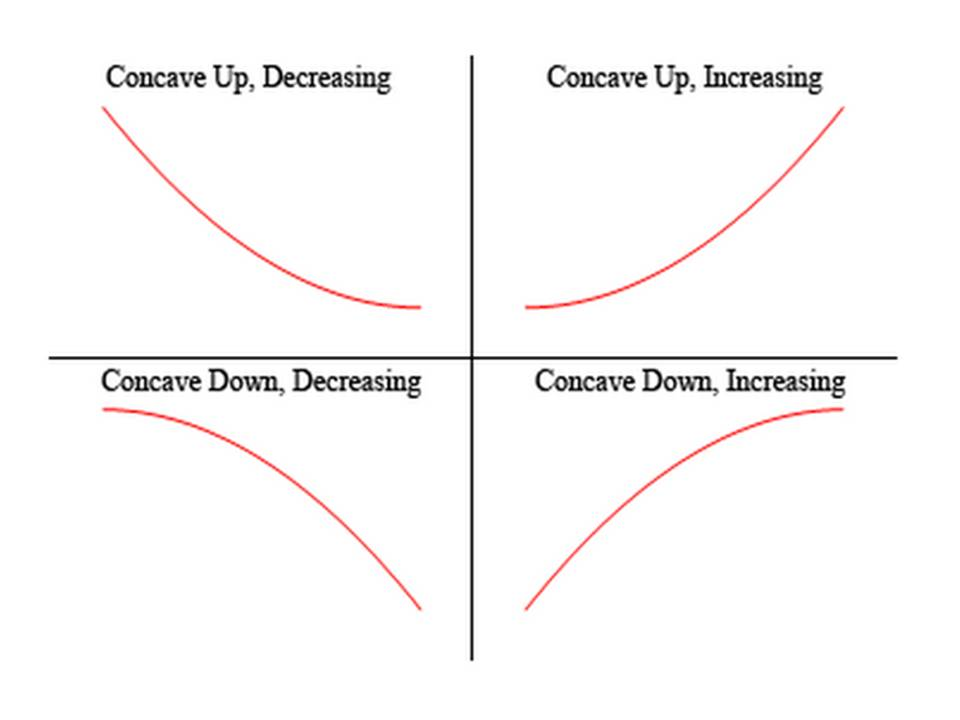
\includegraphics[width=0.99\linewidth]{CurveSketchingGraphs1/Slide5}
\end{figure}

% ShapeOfGraphI_G1
\end{frame}
%================================================================================ %
\begin{frame} 
 \frametitle{Function Concavity}
 So a function is concave up if it “opens” up and the function is concave down if it “opens” down.  Notice as well that concavity has nothing to do with increasing or decreasing.  A function can be concave up and either increasing or decreasing.  Similarly, a function can be concave down and either increasing or decreasing.
 
 It’s probably not the best way to define concavity by saying which way it “opens” since this is a somewhat nebulous definition.  Here is the mathematical definition of concavity.
\end{frame}
 %================================================================================ %
\begin{frame}
 \frametitle{Function Concavity}
 \textbf{ Definition 1 }
 Given the function  then
 
 \begin{itemize}
\item is \textbf{concave up} on an interval \textbf{I} if all of the tangents to the curve on I are below the graph of .
 
\item is \textbf{concave down} on an interval \textbf{I} if all of the tangents to the curve on I are above the graph of .
 \end{itemize}
\end{frame}
%================================================================================ %
\begin{frame} 
	\frametitle{Function Concavity}
 
 To show that the graphs above do in fact have concavity claimed above here is the graph again (blown up a little to make things clearer).
\end{frame}
%================================================================================ %
\begin{frame} 
	\frametitle{Function Concavity}
	 % % ShapeOfGraphI_G2
	 \begin{figure}
\centering
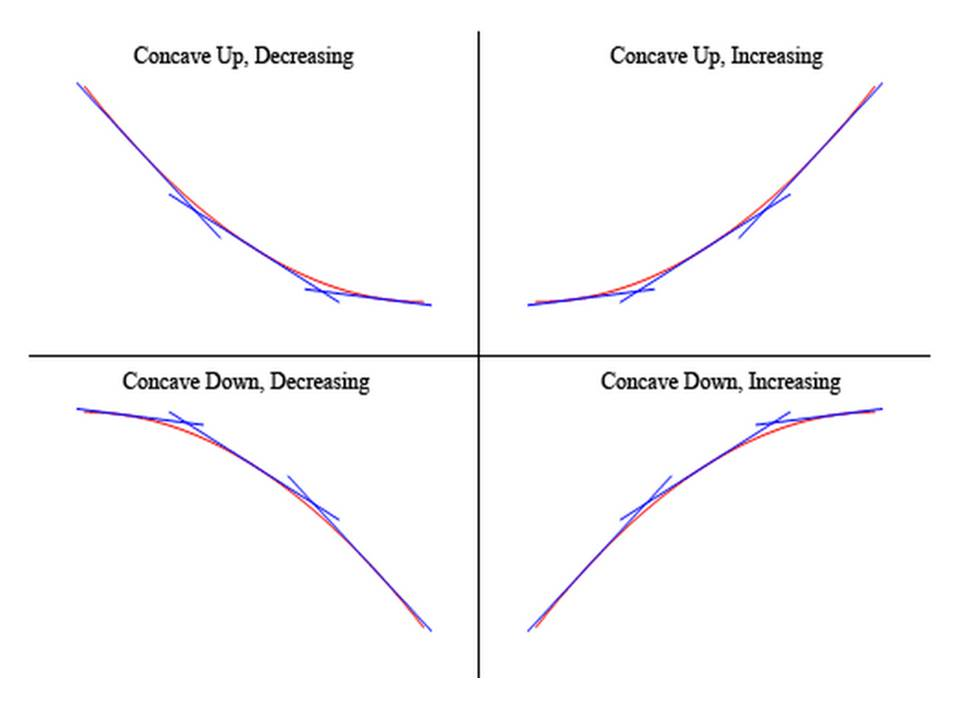
\includegraphics[width=0.99\linewidth]{CurveSketchingGraphs1/Slide6}

\end{figure}

\end{frame}
%================================================================================ %
\begin{frame} 
	\frametitle{Function Concavity}
\begin{itemize}
\item So, as you can see, in the two upper graphs all of the tangent lines sketched in are all below the graph of the function and these are concave up.  
\item In the lower two graphs all the tangent lines are above the graph of the function and these are concave down. 
\end{itemize}
\end{frame}
%================================================================================ %
\begin{frame} 
	\frametitle{Function Concavity}
 \begin{itemize}
 \item Again, notice that concavity and the increasing/decreasing aspect of the function is completely separate and do not have anything to do with the other.  
 \item This is important to note because students often mix these two up and use information about one to get information about the other.
 \end{itemize}

\end{frame}
\section*{Points of Inflection}
%================================================================================ %
\begin{frame} 
	\frametitle{Shape of a Curve}
 There’s one more definition that we need to get out of the way.\\
 
\textbf{Definition 2}
\begin{itemize}
\item A point  is called an inflection point if the function is continuous at the point and the concavity of the graph changes at that point.
\end{itemize}

\end{frame}
%================================================================================ %
\begin{frame} 
	\frametitle{Function Concavity}
	\begin{itemize}
	 \item Now that we have all the concavity definitions out of the way we need to bring the \textbf{second derivative} into the mix.  
	 \item We did after all start off this section saying we were going to be using the second derivative to get information about the graph.  
	 \item The following fact relates the second derivative of a function to its concavity. 
	\end{itemize}

 % The proof of this fact is in the Proofs From Derivative Applications section of the Extras chapter.
\end{frame}
%================================================================================ %
\begin{frame} 
	\frametitle{Function Concavity}
 Fact
 Given the function  then,
 \begin{itemize}
 \item If  for all x in some interval I then  is concave up on I.
  
 \item If  for all x in some interval I then  is concave down on I.
 \end{itemize}

\end{frame}
%================================================================================ %
\begin{frame} 
	\frametitle{Function Concavity}
	\begin{itemize}
	\item  Notice that this fact tells us that a list of possible inflection points will be those points where the second derivative is zero or doesn’t exist.  
	\item Be careful however to not make the assumption that just because the second derivative is zero or doesn’t exist that the point will be an inflection point.  
	\item We will only know that it is an inflection point once we determine the concavity on both sides of it.  
	\item It will only be an inflection point if the concavity is different on both sides of the point.
	\end{itemize}
	
 \end{frame}
 %================================================================================ %
 \begin{frame} 
 	\frametitle{Function Concavity}
 Now that we know about concavity we can use this information as well as the increasing/decreasing information from the previous section to get a pretty good idea of what a graph should look like.  Let’s take a look at an example of that.
\end{frame}
%================================================================================ %
\begin{frame} 
	\frametitle{Function Concavity}
	
\textbf{Example 1}\\ For the following function identify the intervals where the function is increasing and decreasing and the intervals where the function is concave up and concave down.  Use this information to sketch the graph.
 
 
 Solution
 Okay, we are going to need the first two derivatives so let’s get those first.
 
\end{frame}
%================================================================================ %
\begin{frame} 
	\frametitle{Function Concavity}
\begin{itemize}
\item Let’s start with the increasing/decreasing information since we should be fairly comfortable with that after the last section.
 
\item There are three critical points for this function : ,  , and .  
\item Below is the number line for the increasing/decreasing information.
\end{itemize}

\end{frame}
%================================================================================ %
\begin{frame} 
\frametitle{Function Concavity}
\begin{figure}
\centering
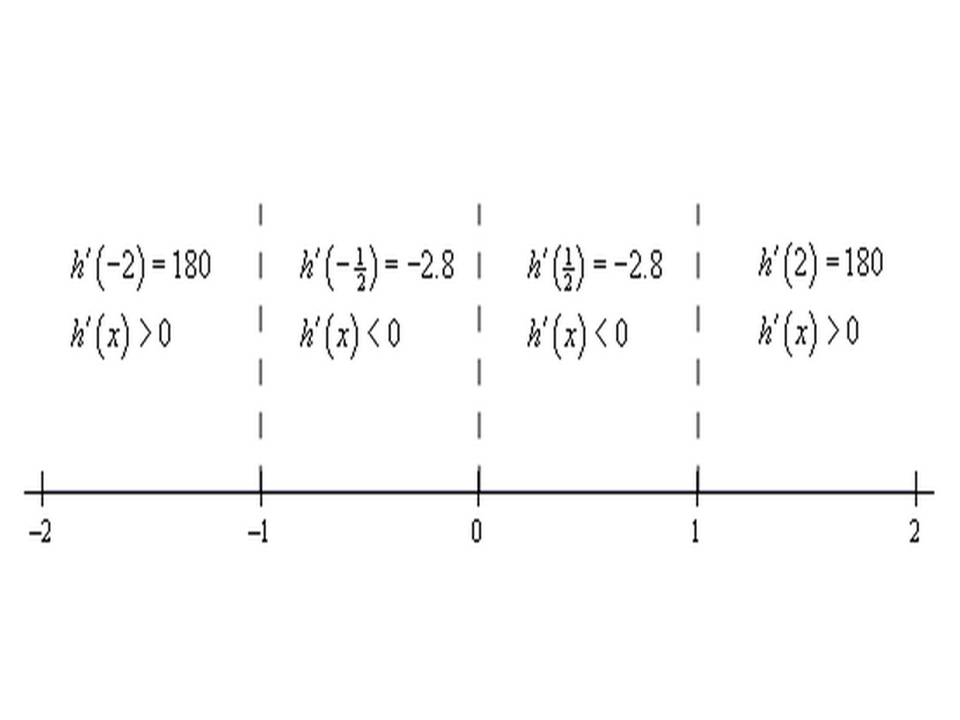
\includegraphics[width=0.99\linewidth]{CurveSketchingGraphs1/Slide7}
\caption{}
\label{fig:Slide7}
\end{figure}



\end{frame}
%================================================================================ %
\begin{frame} 
	\frametitle{Function Concavity}
% % ShapeOfGraphII_Ex1_G1
 
 So, it looks like we’ve got the following intervals of increasing and decreasing.
 
 
 Note that from the first derivative test we can also say that  is a relative maximum and that  is a relative minimum.  Also  is neither a relative minimum or maximum.
\end{frame}
%================================================================================ %
\begin{frame} 
	\frametitle{Function Concavity}
 Now let’s get the intervals where the function is concave up and concave down.  If you think about it this process is almost identical to the process we use to identify the intervals of increasing and decreasing.  This only difference is that we will be using the second derivative instead of the first derivative.
\end{frame}
%================================================================================ %
\begin{frame} 
	\frametitle{Function Concavity} 
 The first thing that we need to do is identify the possible inflection points.  These will be where the second derivative is zero or doesn’t exist.  The second derivative in this case is a polynomial and so will exist everywhere.  It will be zero at the following points.
 
\end{frame}
%================================================================================ %
\begin{frame} 
	\frametitle{Function Concavity}
 As with the increasing and decreasing part we can draw a number line up and use these points to divide the number line into regions.  In these regions we know that the second derivative will always have the same sign since these three points are the only places where the function may change sign.  Therefore, all that we need to do is pick a point from each region and plug it into the second derivative.  
 
\end{frame}
%================================================================================ %
\begin{frame} 
	\frametitle{Function Concavity}The second derivative will then have that sign in the whole region from which the point came from
 
 Here is the number line for this second derivative.
% % ShapeOfGraphII_Ex1_G2
\end{frame}
%================================================================================ %
\begin{frame} 
	\frametitle{Function Concavity} 
 So, it looks like we’ve got the following intervals of concavity.
 
\end{frame}
%================================================================================ %
\begin{frame} 
	\frametitle{Function Concavity} 
 This also means that
 
 are all inflection points.
\end{frame}
%================================================================================ %
\begin{frame} 
	\frametitle{Function Concavity} 
 All this information can be a little overwhelming when going to sketch the graph.  The first thing that we should do is get some starting points.  The critical points and inflection points are good starting points.  So, first graph these points.  Now, start to the left and start graphing the increasing/decreasing information as we did in the previous section when all we had was the increasing/decreasing information.  As we graph this we will make sure that the concavity information matches up with what we’re graphing.
\end{frame}
%================================================================================ %
\begin{frame} 
	\frametitle{Function Concavity}
 Using all this information to sketch the graph gives the following graph.
\begin{figure}
\centering
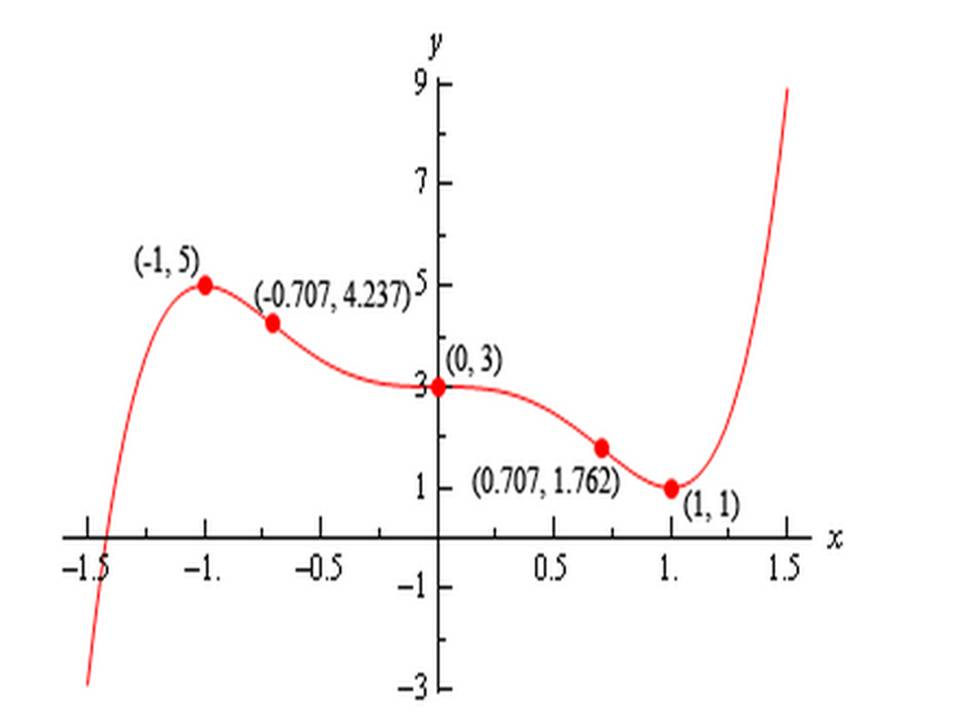
\includegraphics[width=0.79\linewidth]{CurveSketchingGraphs1/Slide9}

\end{figure}
\end{frame}
%================================================================================ %
\begin{frame} 
	\frametitle{Function Concavity}
 
 We can use the previous example to illustrate another way to classify some of the critical points of a function as relative maximums or relative minimums.
\end{frame}
%================================================================================ %
\begin{frame} 
	\frametitle{Function Concavity} 
 Notice that  is a relative maximum and that the function is concave down at this point. This means that  must be negative.  Likewise,  is a relative minimum and the function is concave up at this point.  This means that  must be positive. 
 
 As we’ll see in a bit we will need to be very careful with .  In this case the second derivative is zero, but that will not actually mean that  is not a relative minimum or maximum.  We’ll see some examples of this in a bit, but we need to get some other information taken care of first.
\end{frame}
%================================================================================ %
\begin{frame} 
	\frametitle{Function Concavity} 
 It is also important to note here that all of the critical points in this example were critical points in which the first derivative was zero and this is required for this to work.  We will not be able to use this test on critical points where the derivative doesn’t exist.
\end{frame}
%================================================================================ %
\begin{frame} 
	\frametitle{Function Concavity}
\begin{itemize}
\item Here is the test that can be used to classify some of the critical points of a function.  
\item The proof of this test is in the Proofs From Derivative Applications section of the Extras chapter.
\end{itemize}

\end{frame}
%================================================================================ %
\begin{frame} 
\frametitle{Second Derivative Test} 
\textbf{ Second Derivative Test }\\
 Suppose that  is a critical point of  such that  and that  is continuous in a region around .  Then,
 \begin{itemize}
\item If  then  is a relative maximum.
\item If  then  is a relative minimum.
\item If  then  can be a relative maximum, relative minimum or neither.
\end{itemize}
\end{frame}
%================================================================================ %
\begin{frame} 
\frametitle{Second Derivative Test} 
 The third part of the second derivative test is important to notice.  If the second derivative is zero then the critical point can be anything.  Below are the graphs of three functions all of which have a critical point at , the second derivative of all of the functions is zero at  and yet all three possibilities are exhibited.
\end{frame}
%================================================================================ %
\begin{frame} 
\frametitle{Second Derivative Test} 
 The first is the graph of .  This graph has a relative minimum at .
 % % ShapeOfGraphII_G1
 
 Next is the graph of  which has a relative maximum at .
 % % ShapeOfGraphII_G2
 
 Finally, there is the graph of  and this graph had neither a relative minimum or a relative maximum at .
 % % ShapeOfGraphII_G3
\end{frame}
%================================================================================ %
\begin{frame} 
\frametitle{Second Derivative Test} 
 So, we can see that we have to be careful if we fall into the third case.  For those times when we do fall into this case we will have to resort to other methods of classifying the critical point.  This is usually done with the first derivative test.
 
 Let’s go back and relook at the critical points from the first example and use the Second Derivative Test on them, if possible.
\end{frame}
\end{document}